\section{Circuito Objetivo (Caso 1)}

El primer caso que se analizó es un filtro activo con Amplificadores operacionales. A continuación se muestra su esquemático y los valores de los elementos.

\begin{figure}[H]
\centering
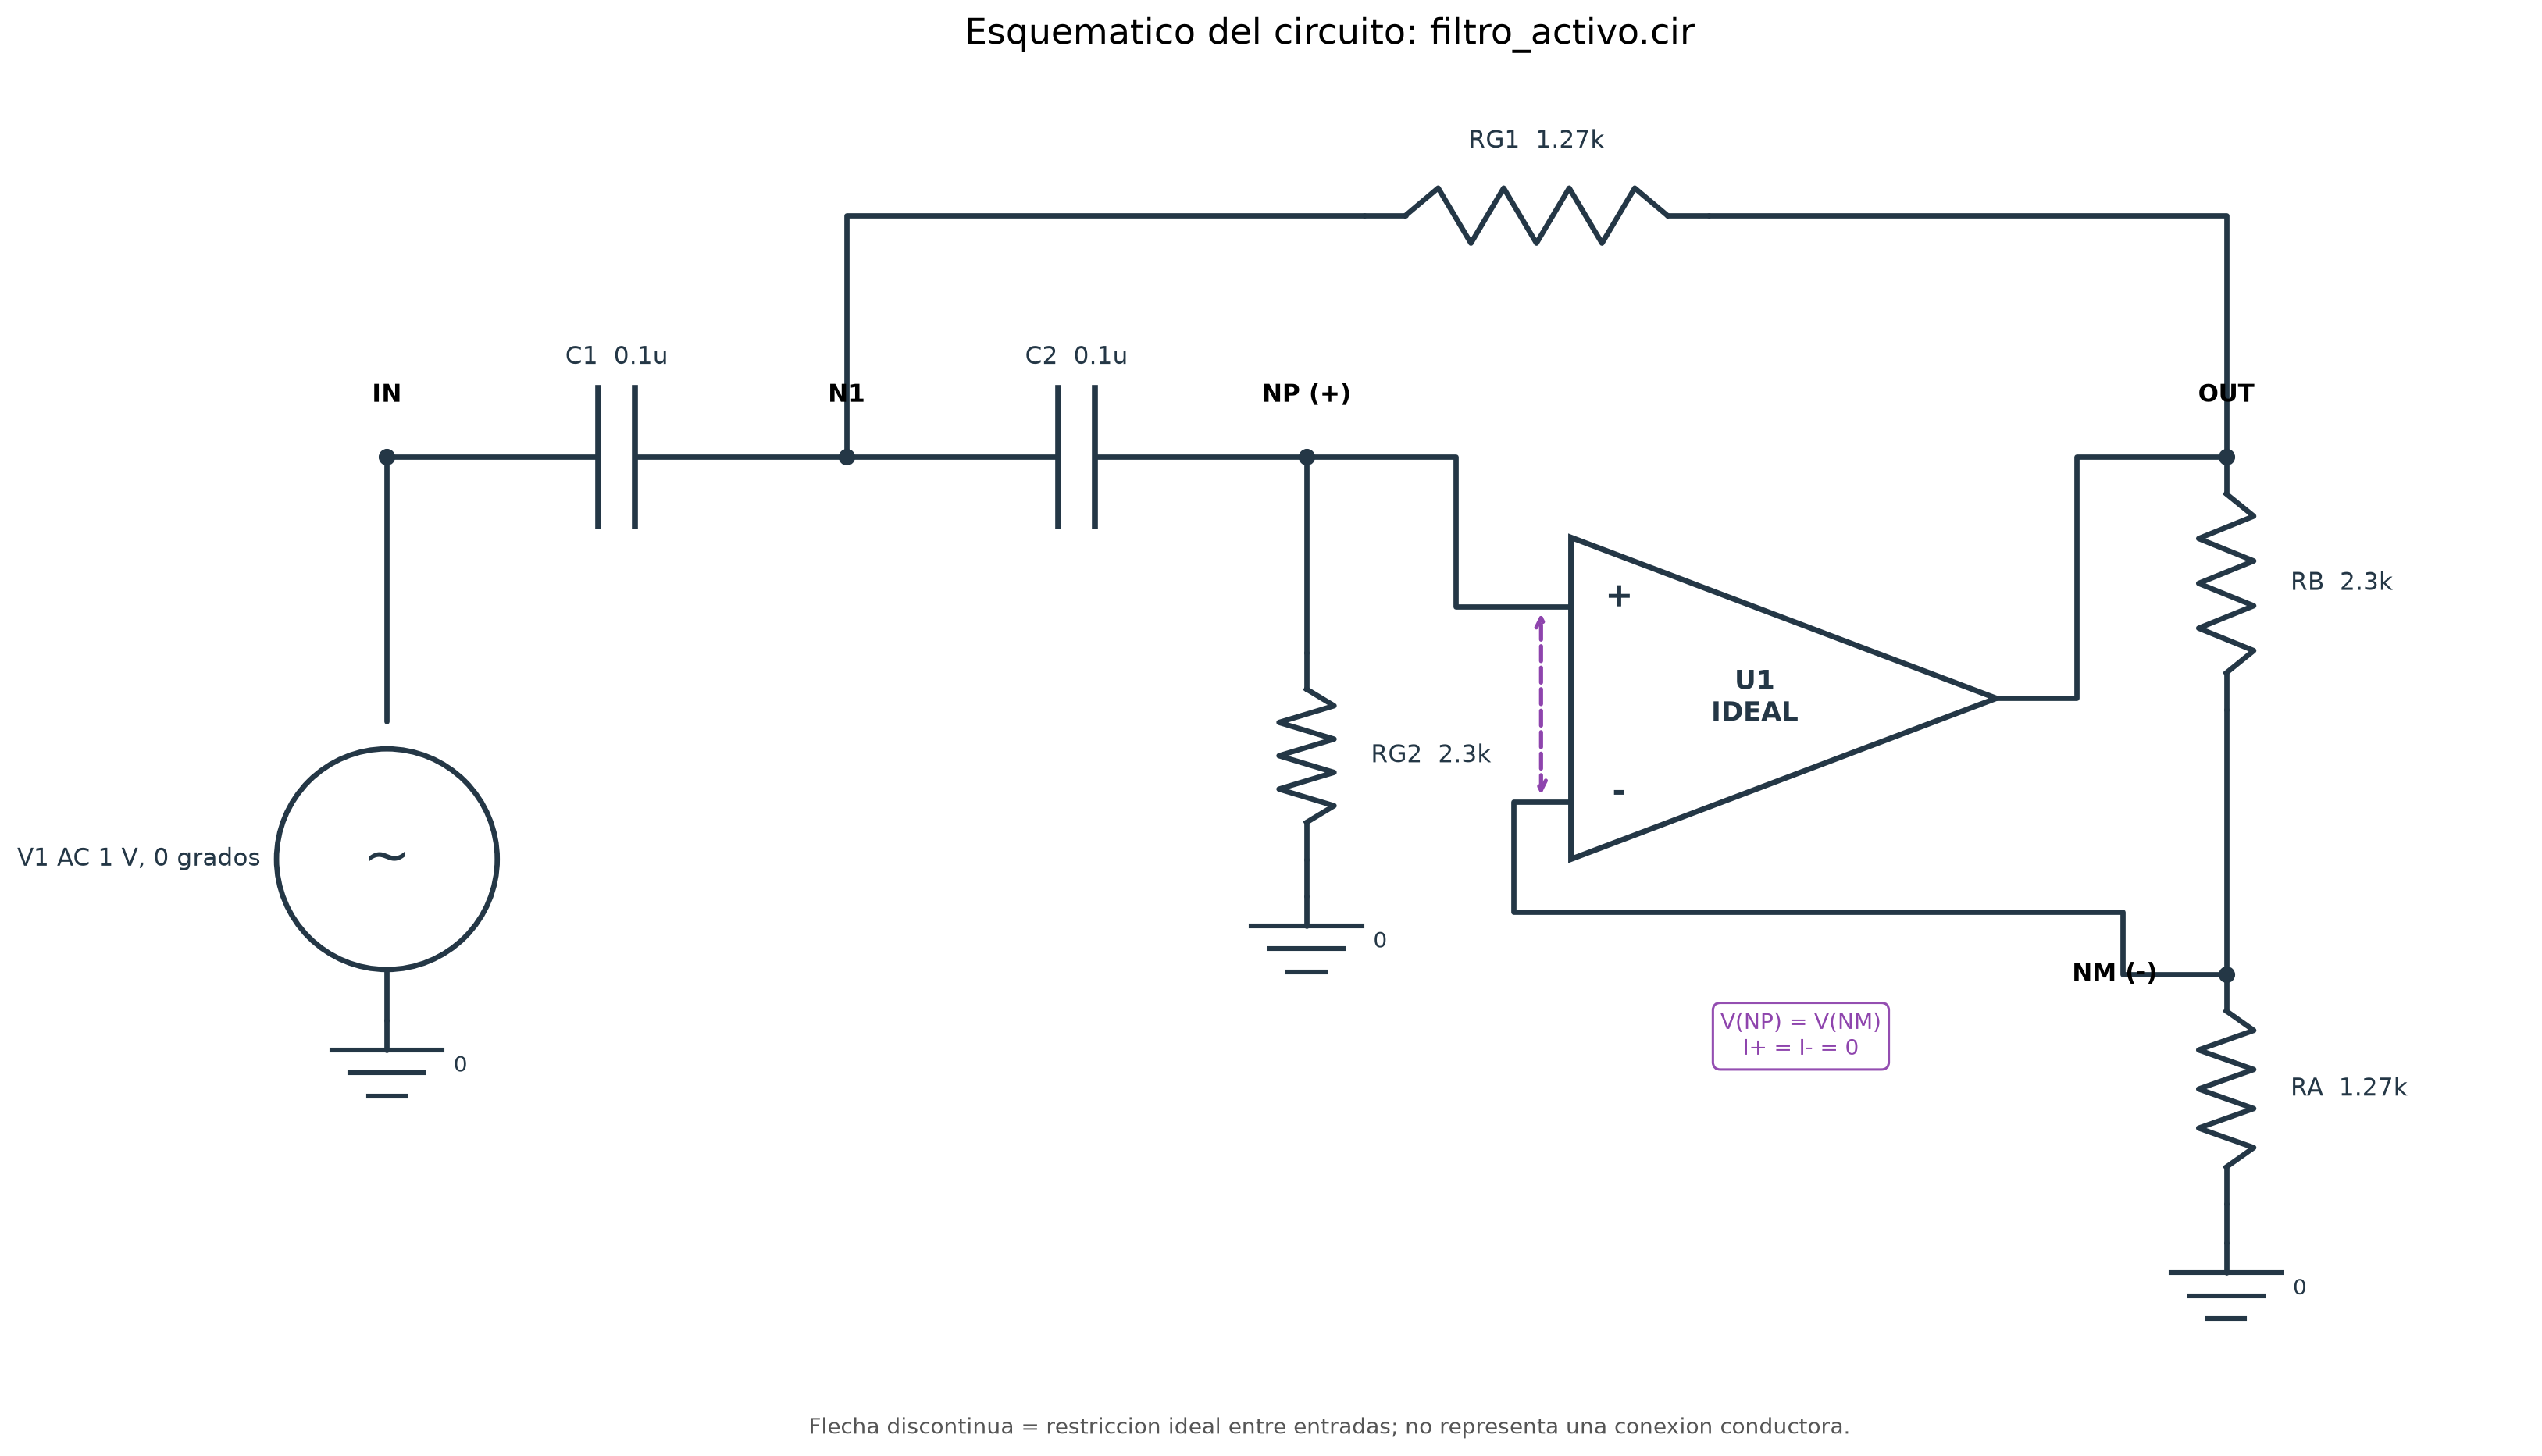
\includegraphics[width=0.8\linewidth]{1_circuito_objetivo_agent/plots/esquematico_filtro_activo.png}
\caption{Esquemático del circuito objetivo.}
\end{figure}

\begin{table}[H]
\centering
\begin{tabular}{ll}
\toprule
Parámetro & Valor \\
\midrule
Frecuencia de inicio & 10 Hz \\
Frecuencia final & 100 kHz \\
Tipo de barrido & Lineal, 300 puntos \\
Fuente AC de entrada & 1 V \\
$C_1$, $C_2$ & 0.1 $\mu$F \\
$R_A$ & 1.27 k$\Omega$ \\
$R_B$ & 2.3 k$\Omega$ \\
$R_G1$ & 1.27 k$\Omega$ \\
$R_G2$ & 2.3 k$\Omega$ \\
Modelo del op-amp & Ideal, extensión MNA del proyecto \\
\bottomrule
\end{tabular}
\caption{Parámetros de simulación del circuito objetivo.}
\end{table}

\subsection{Resultados del analisis en AC del Agente y HSPICE}

La herramienta proporcionó el siguiente análisis de grafos:
\begin{figure}[H]
\centering
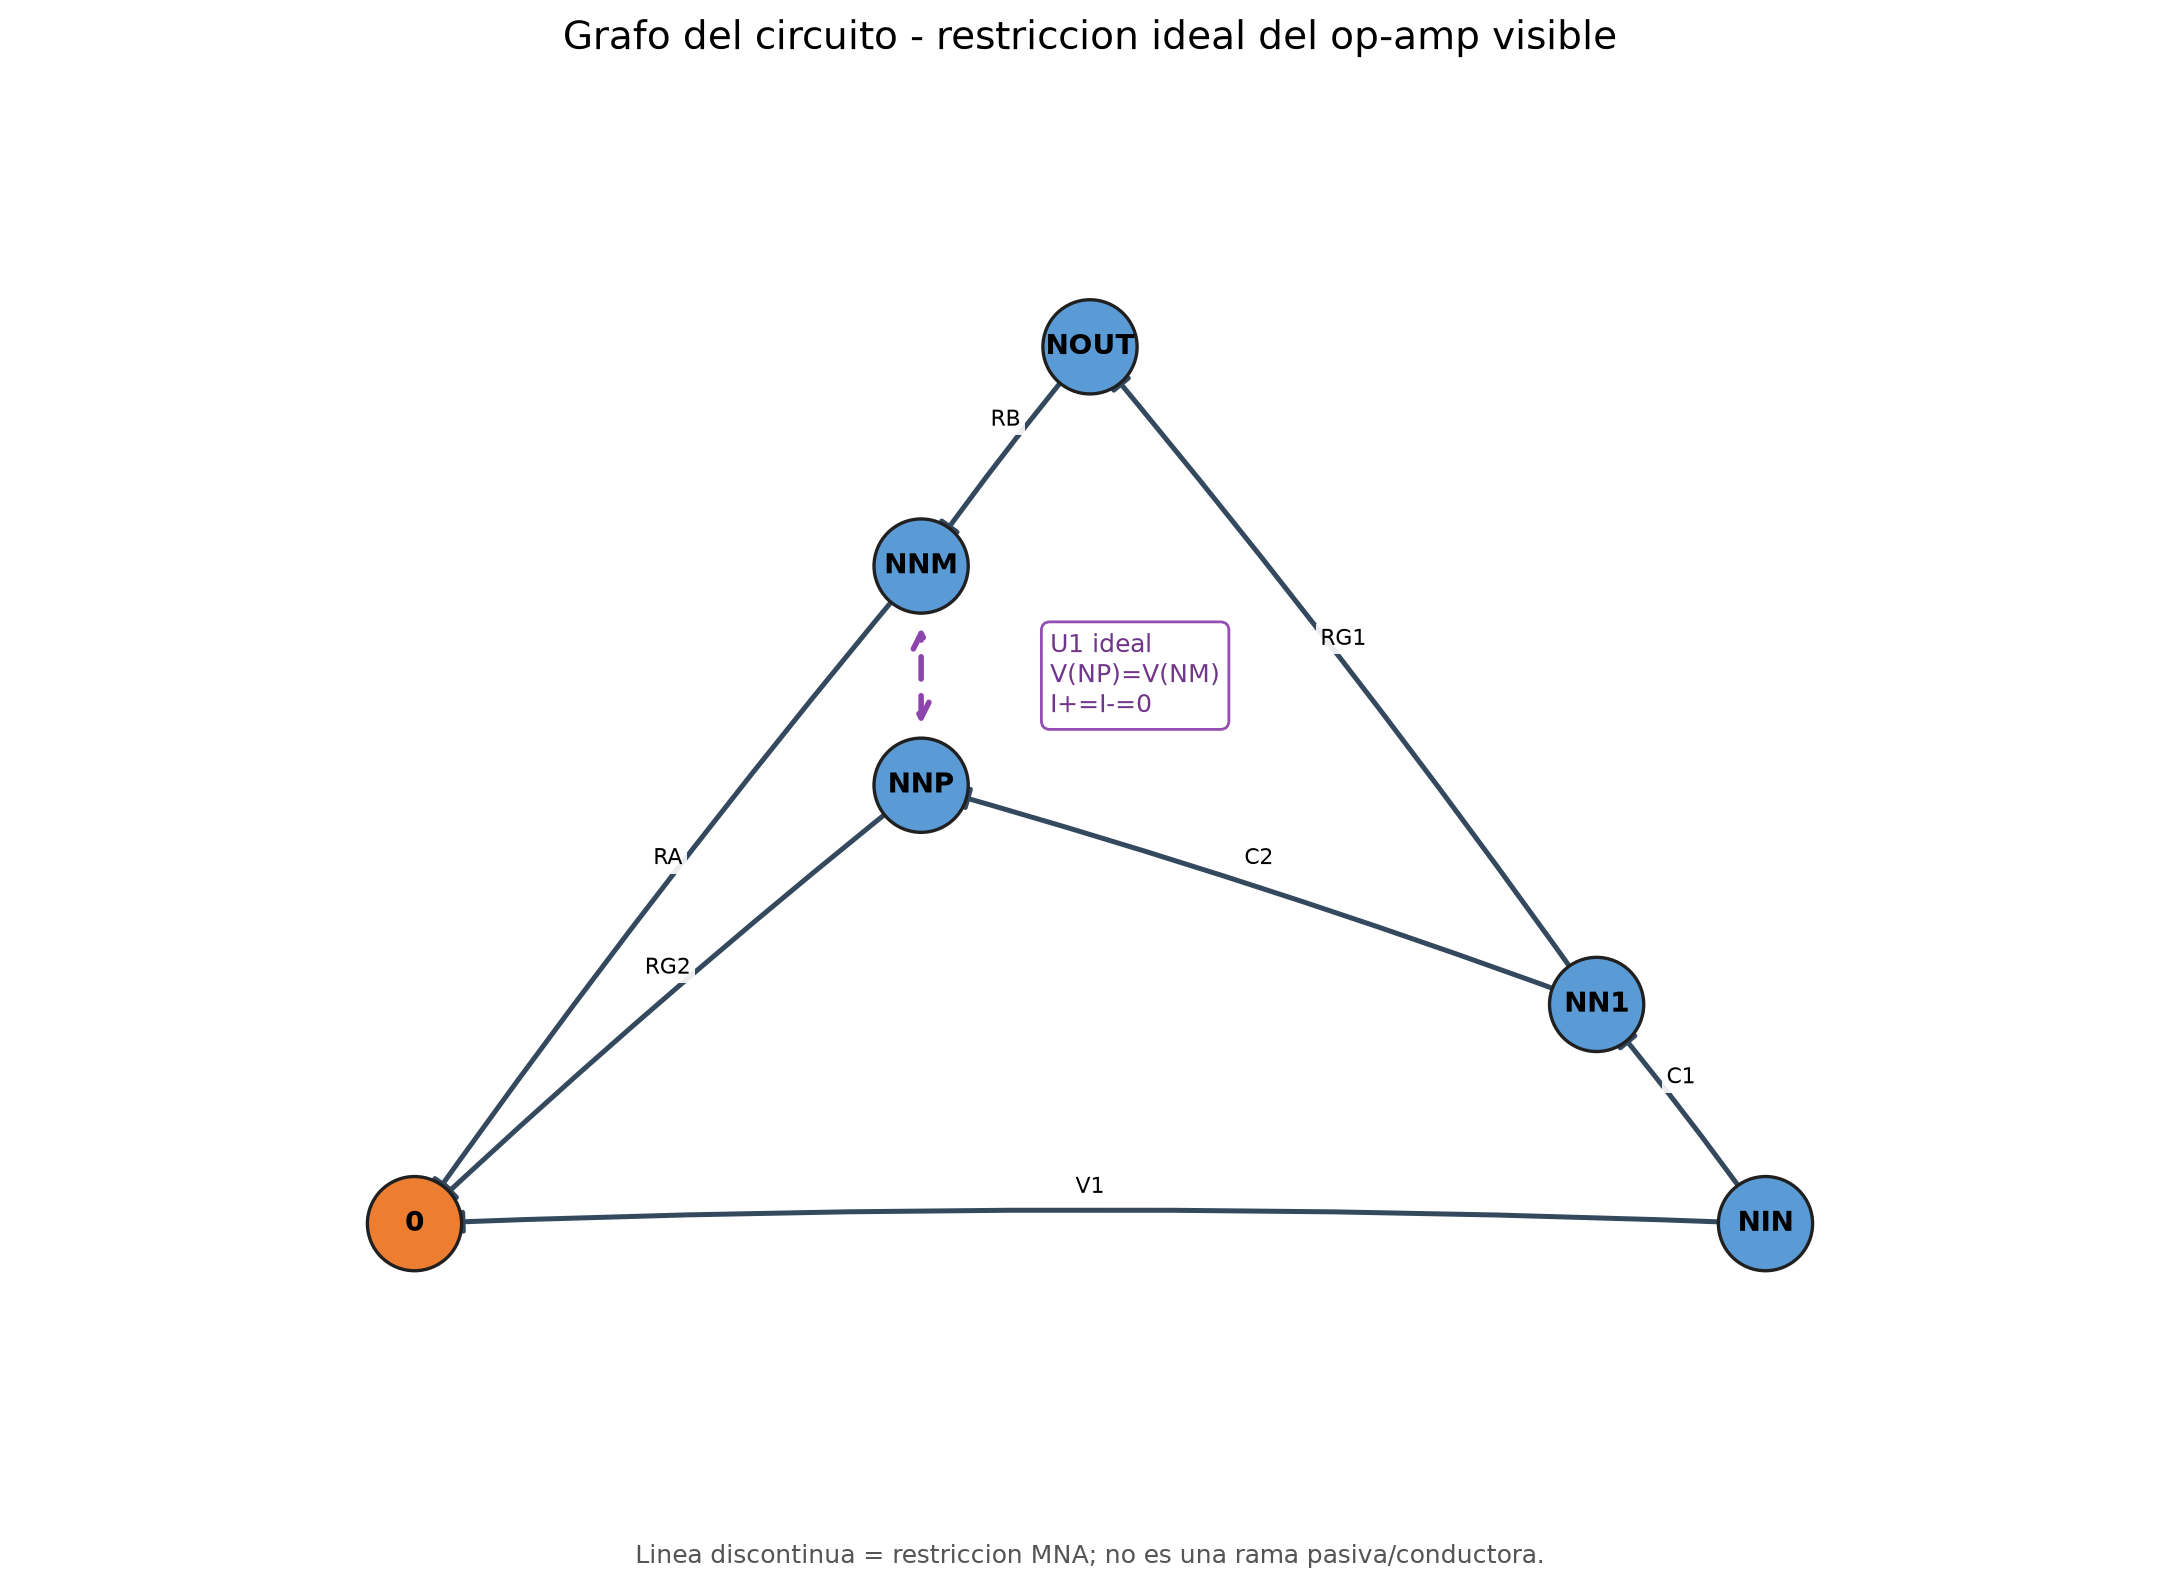
\includegraphics[width=0.8\linewidth]{1_circuito_objetivo_agent/plots/graph.png}
\caption{Análisis de grafos del circuito objetivo.}
\end{figure}

Parte del análisis que genera incluye la formulación de la matriz de Tableua. Nota: El agente no pudo formular completamente la matriz de Tableua, la matriz mostrada a continuación no muestra el elemento del OpAmp, de acuerdo con el agente el analisis MNA cubre lo correspondiente al OpAmp.

\begin{figure}[H]
\centering
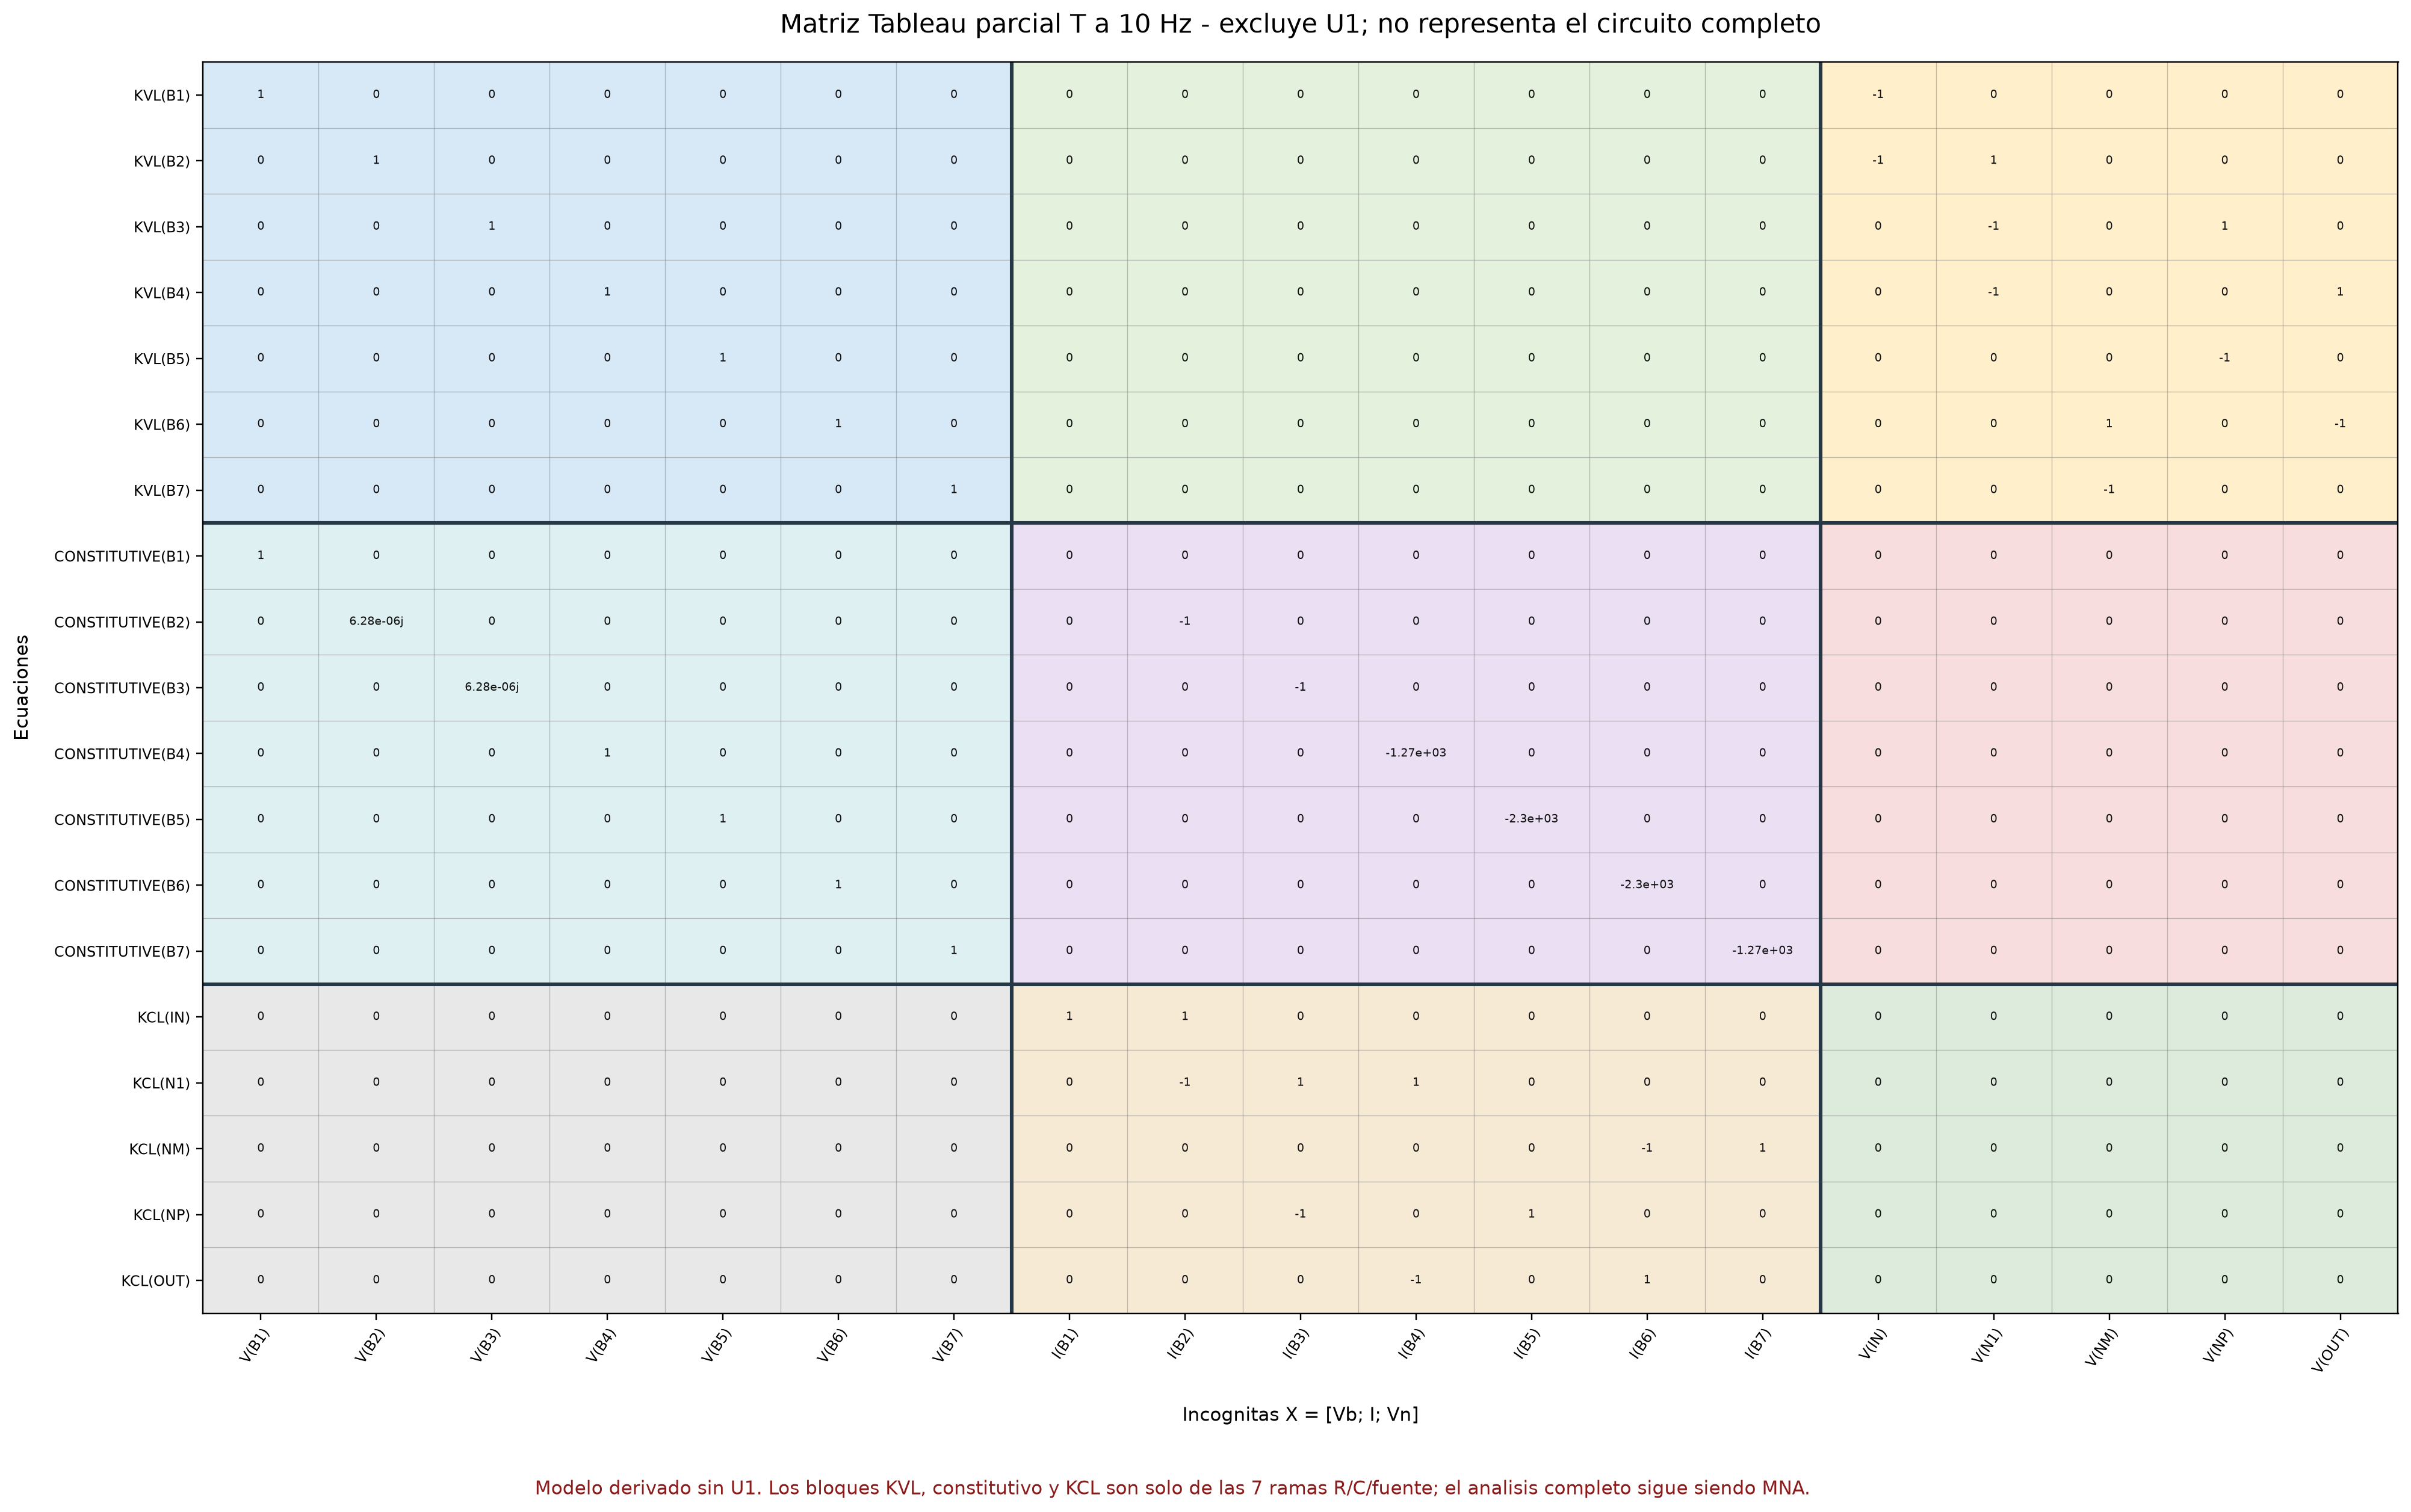
\includegraphics[width=0.8\linewidth]{1_circuito_objetivo_agent/plots/tableau_partial_T_colored_blocks_10Hz.png}
\caption{Matriz de Tableua del circuito objetivo.}
\end{figure}

\begin{figure}[H]
\centering
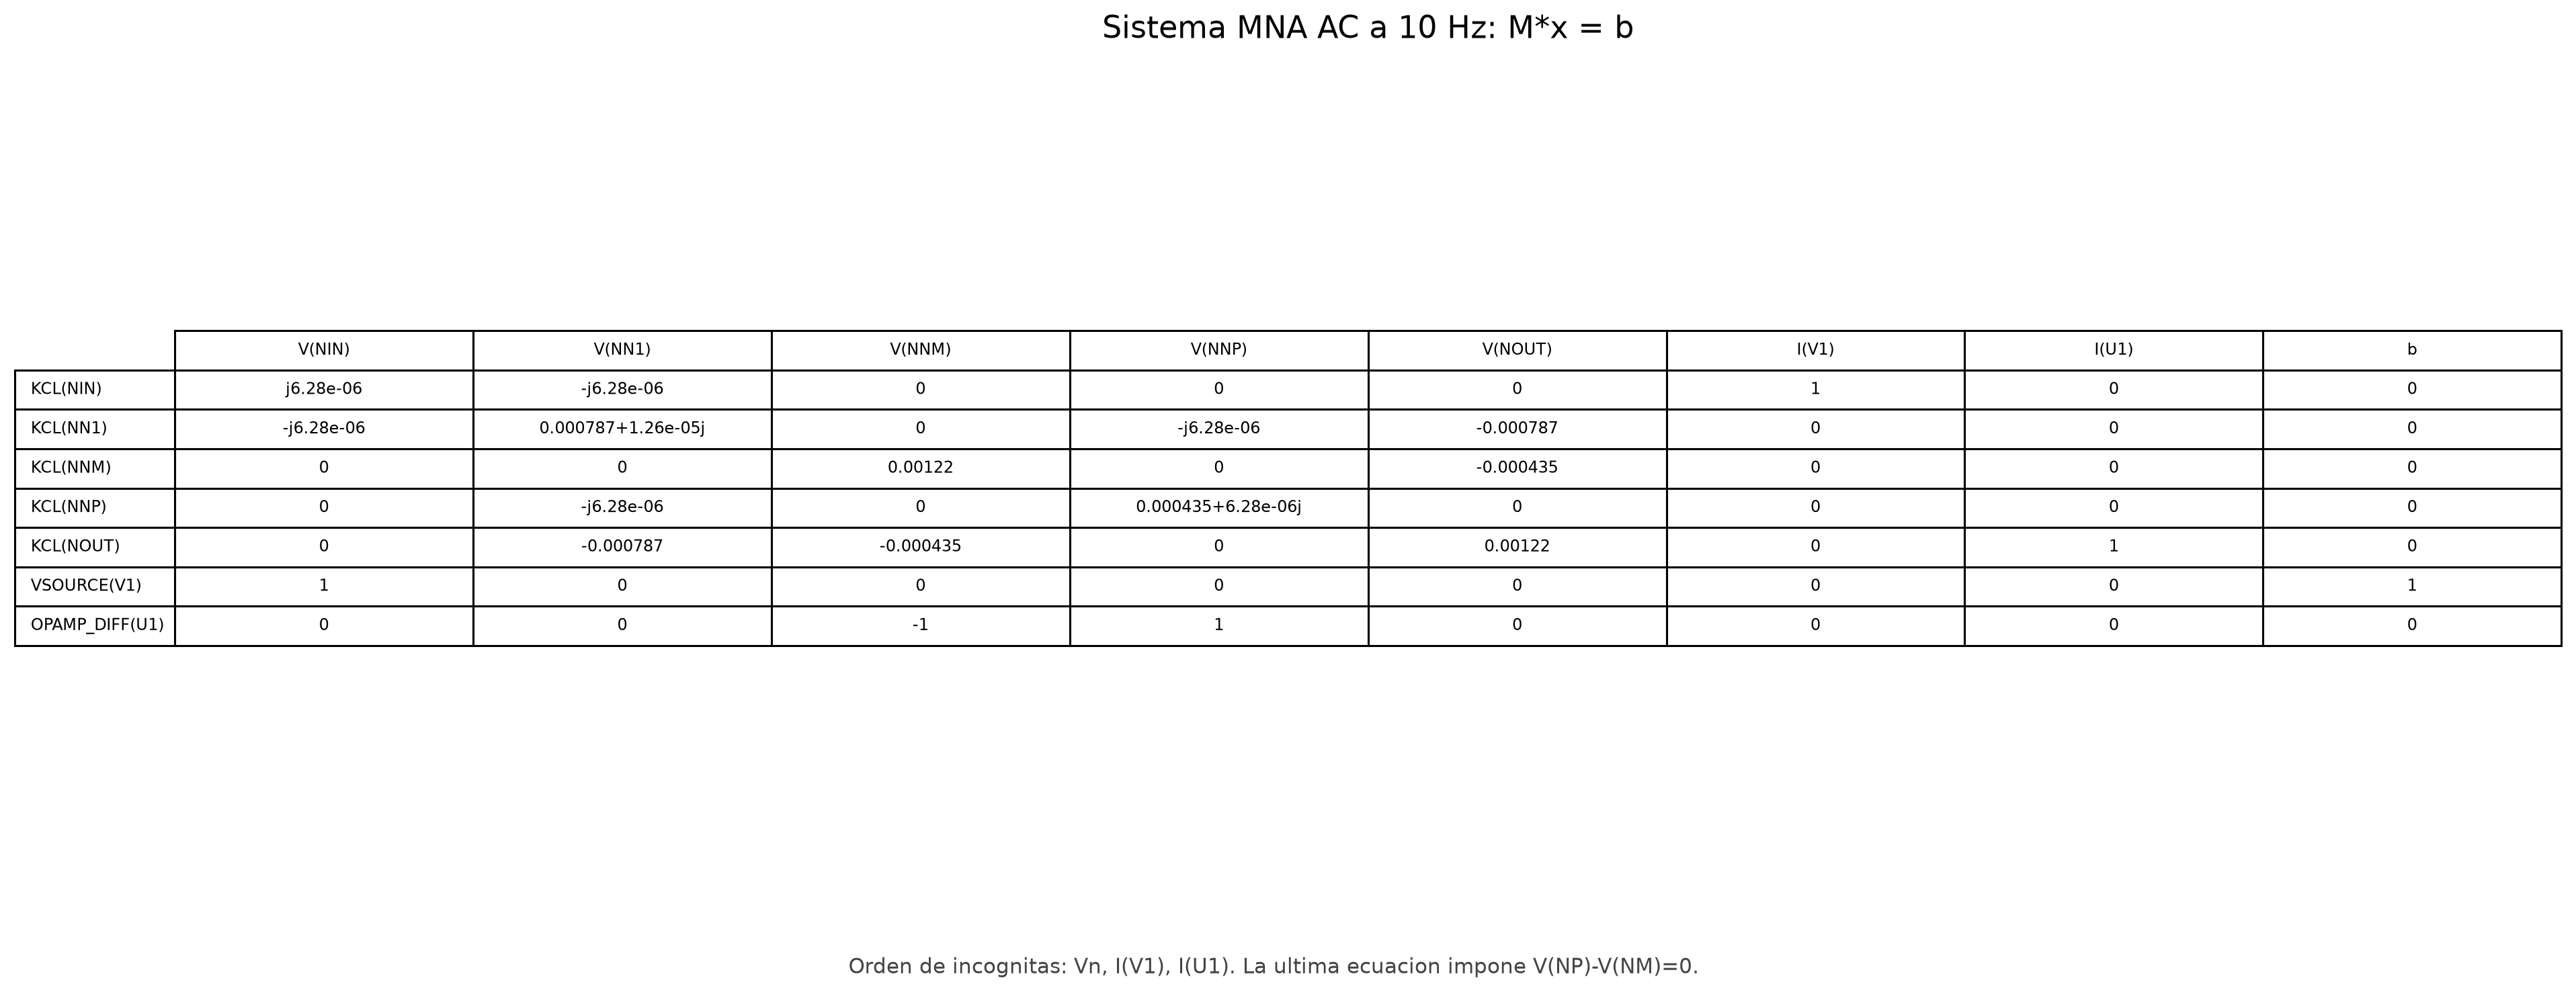
\includegraphics[width=0.95\linewidth]{1_circuito_objetivo_agent/plots/mna_system_10Hz.png}
\caption{Sistema MNA AC completo del circuito a 10 Hz.}
\end{figure}

La herramienta del proyecto reportó un estado general \textbf{Satisfactorio} para el barrido entero. La transferencia se evaluó como $V(NOUT)/V(NIN)$, con validación de cada punto y estado global de la ejecución correcto.

\begin{table}[H]
\centering
\begin{tabular}{lrrr}
\toprule
Punto & Frecuencia (Hz) & $|H(j\omega)|$ & Fase ($^\circ$) \\
\midrule
Inicio & 10 & 0.0003241778 & -179.4148 \\
Punto de máximo local & 1347.6589 & 3.3482009 & -51.5098 \\
Fin & 100000 & 2.8111572 & -0.5074 \\
\bottomrule
\end{tabular}
\caption{Valores representativos del análisis AC del agente SPICE educativo.}
\end{table}

\begin{figure}[H]
\centering
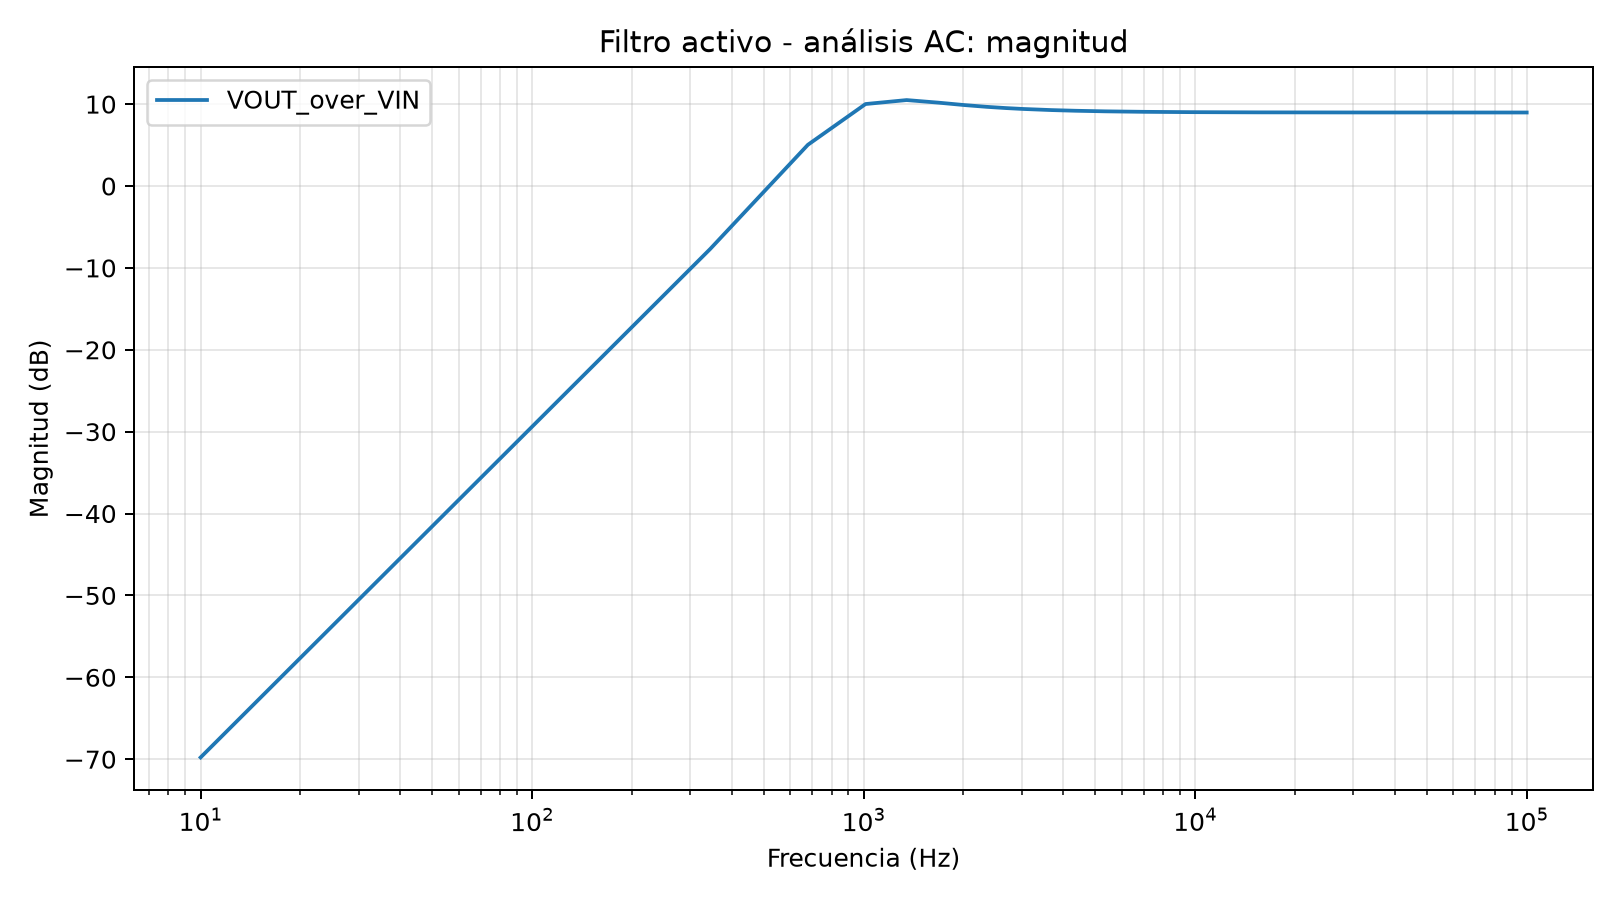
\includegraphics[width=0.8\linewidth]{1_circuito_objetivo_agent/plots/magnitude.png}
\caption{Gráfica de Magnitud en dB de la función de transferencia $H(w)$ obtenida por el agente.}
\end{figure}

\begin{figure}[H]
\centering
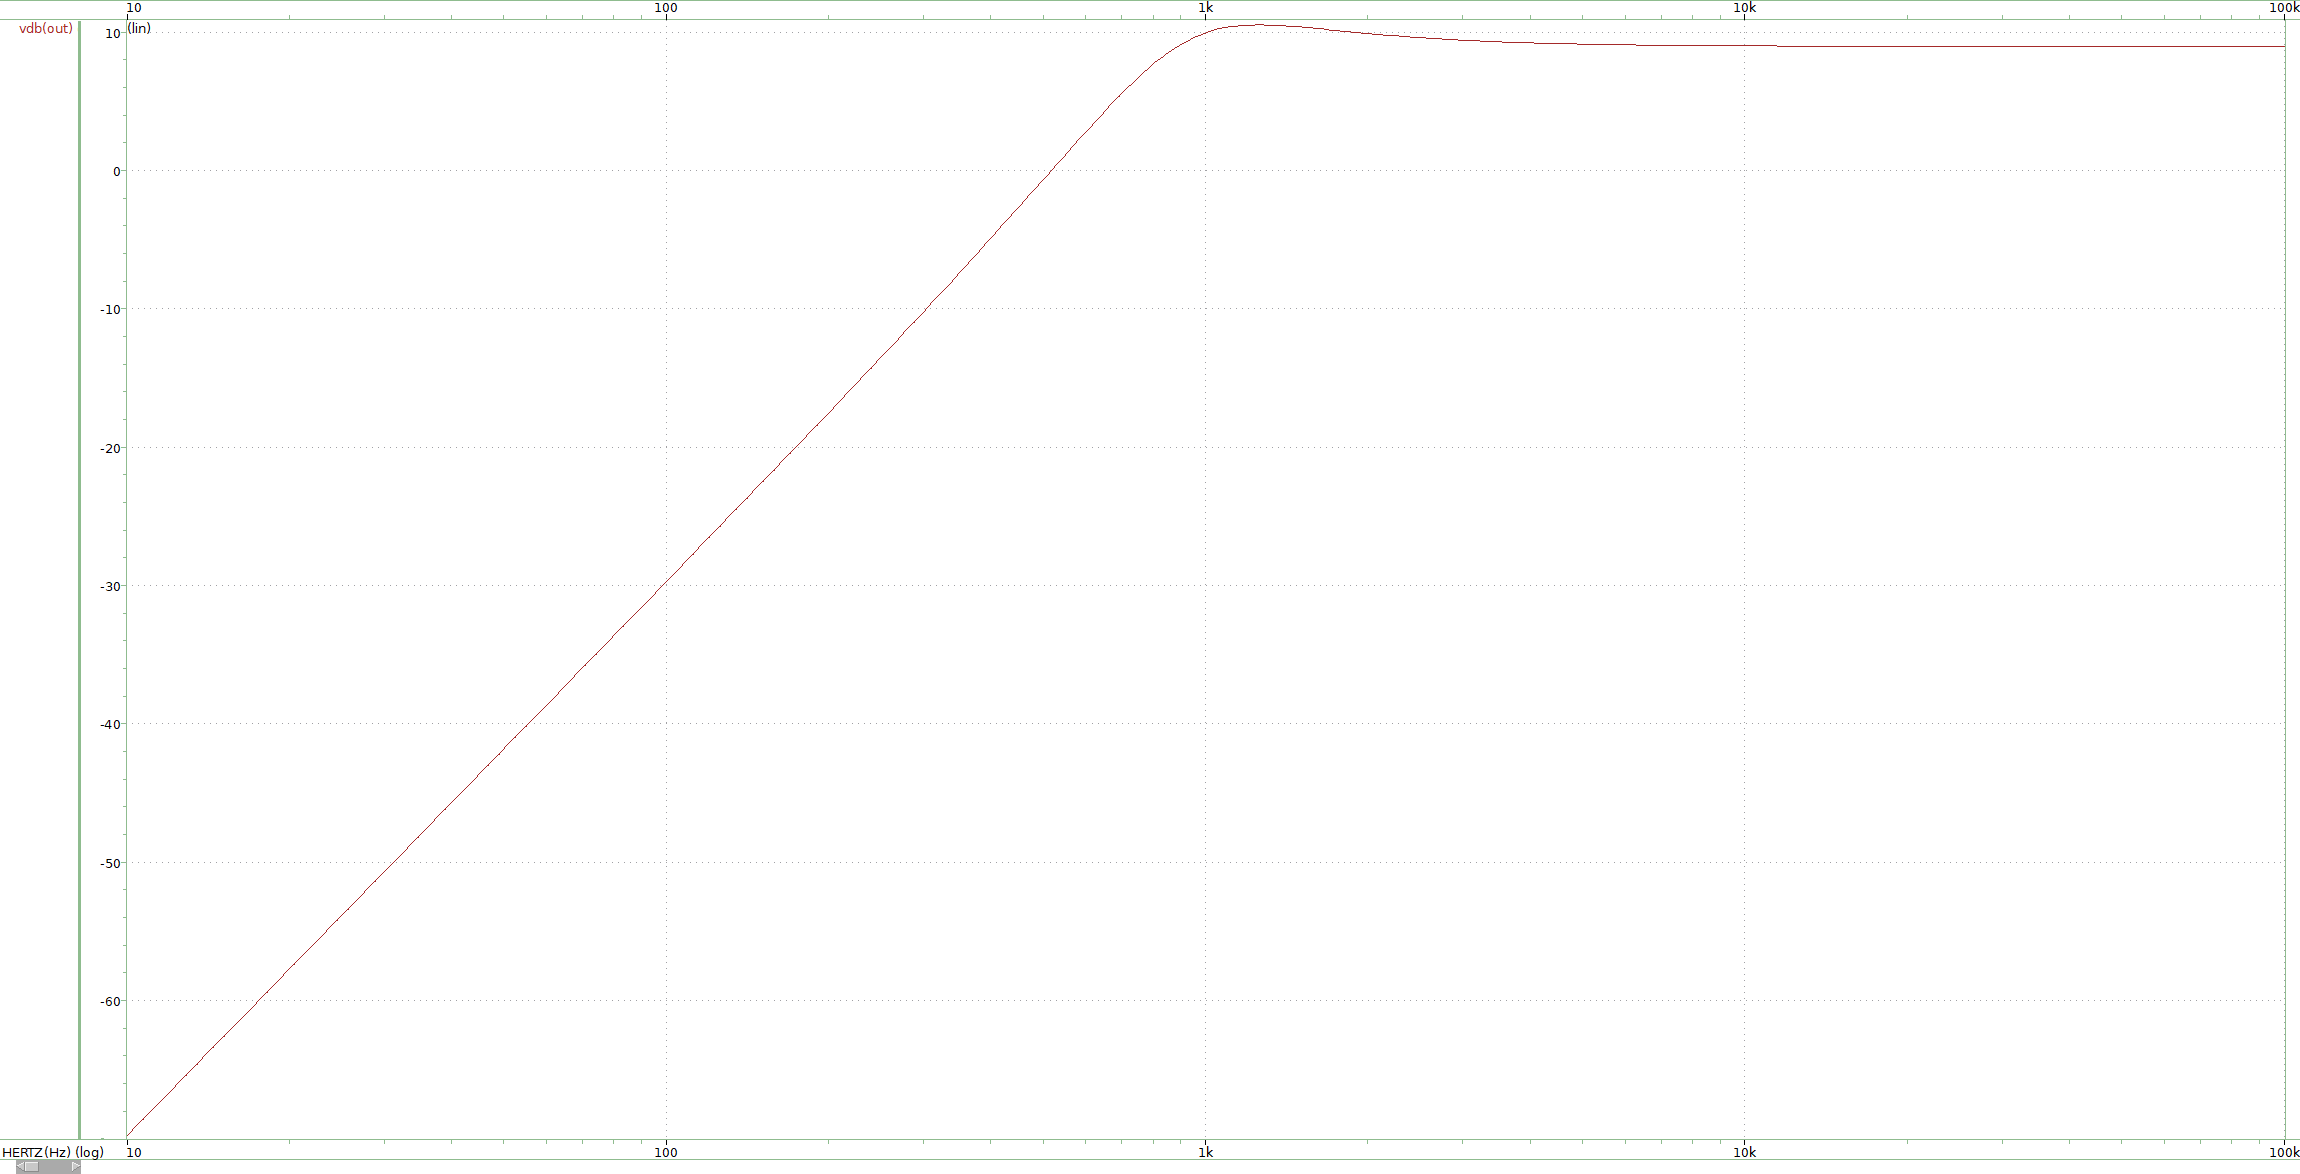
\includegraphics[width=0.8\linewidth]{1_circuito_objetivo_HSPICE/magnitude_dB_hspice.png}
\caption{Gráfica de Magnitud en dB de la función de transferencia $H(w)$ obtenida por HSPICE.}
\end{figure}

\begin{figure}[H]
\centering
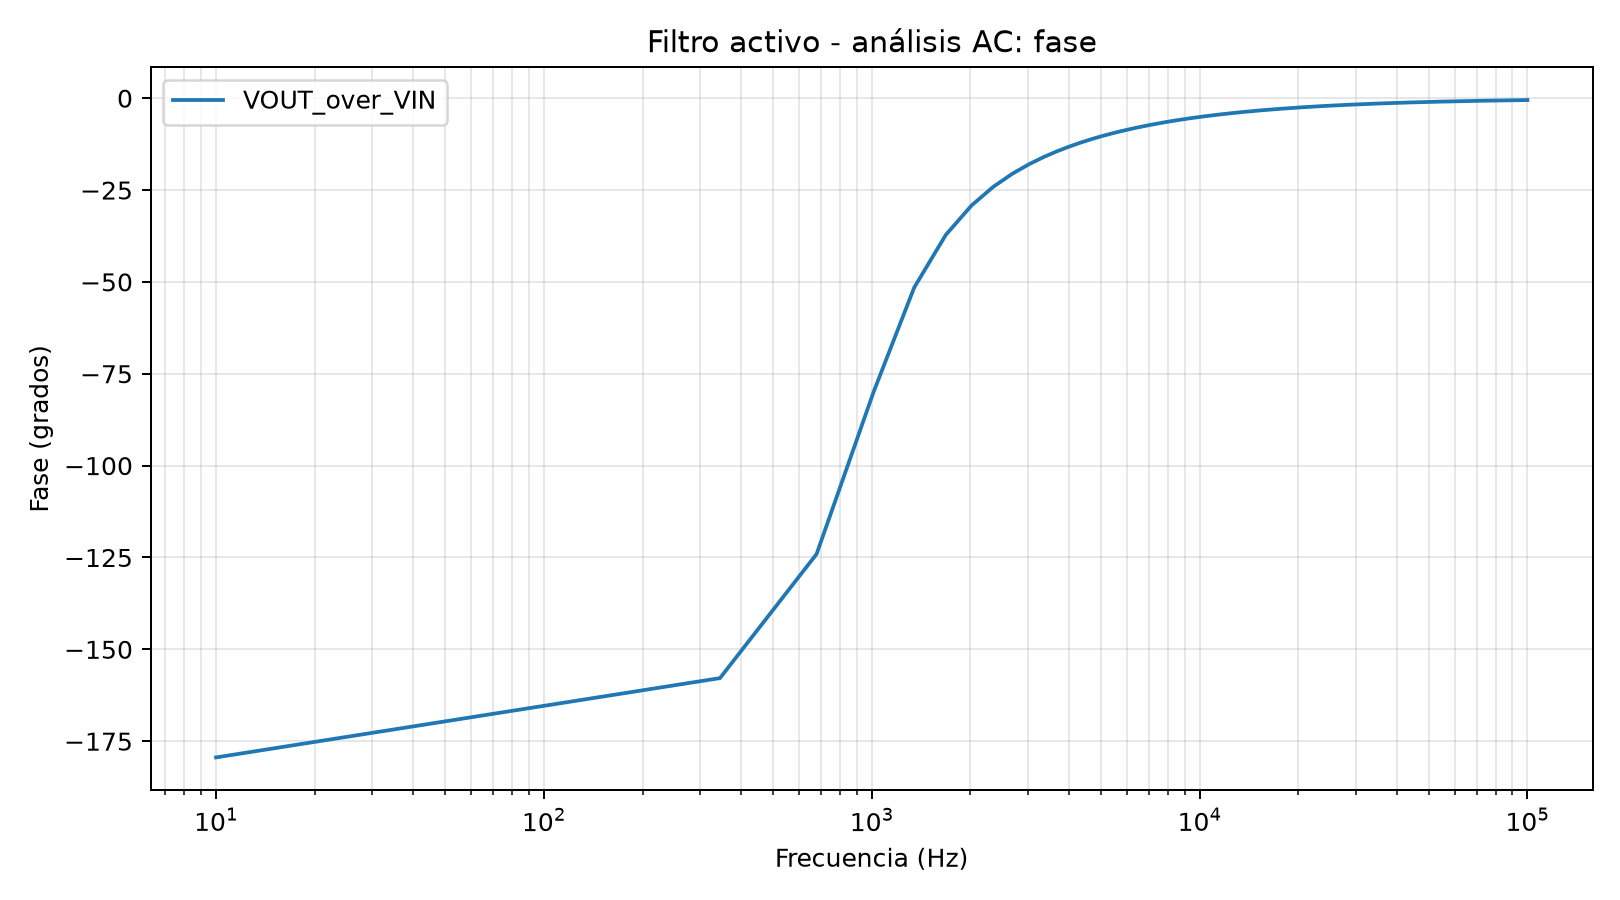
\includegraphics[width=0.8\linewidth]{1_circuito_objetivo_agent/plots/phase.png}
\caption{Gráfica de Fase de la función de transferencia $H(w)$ obtenida por el agente.}
\end{figure}

\begin{figure}[H]
\centering
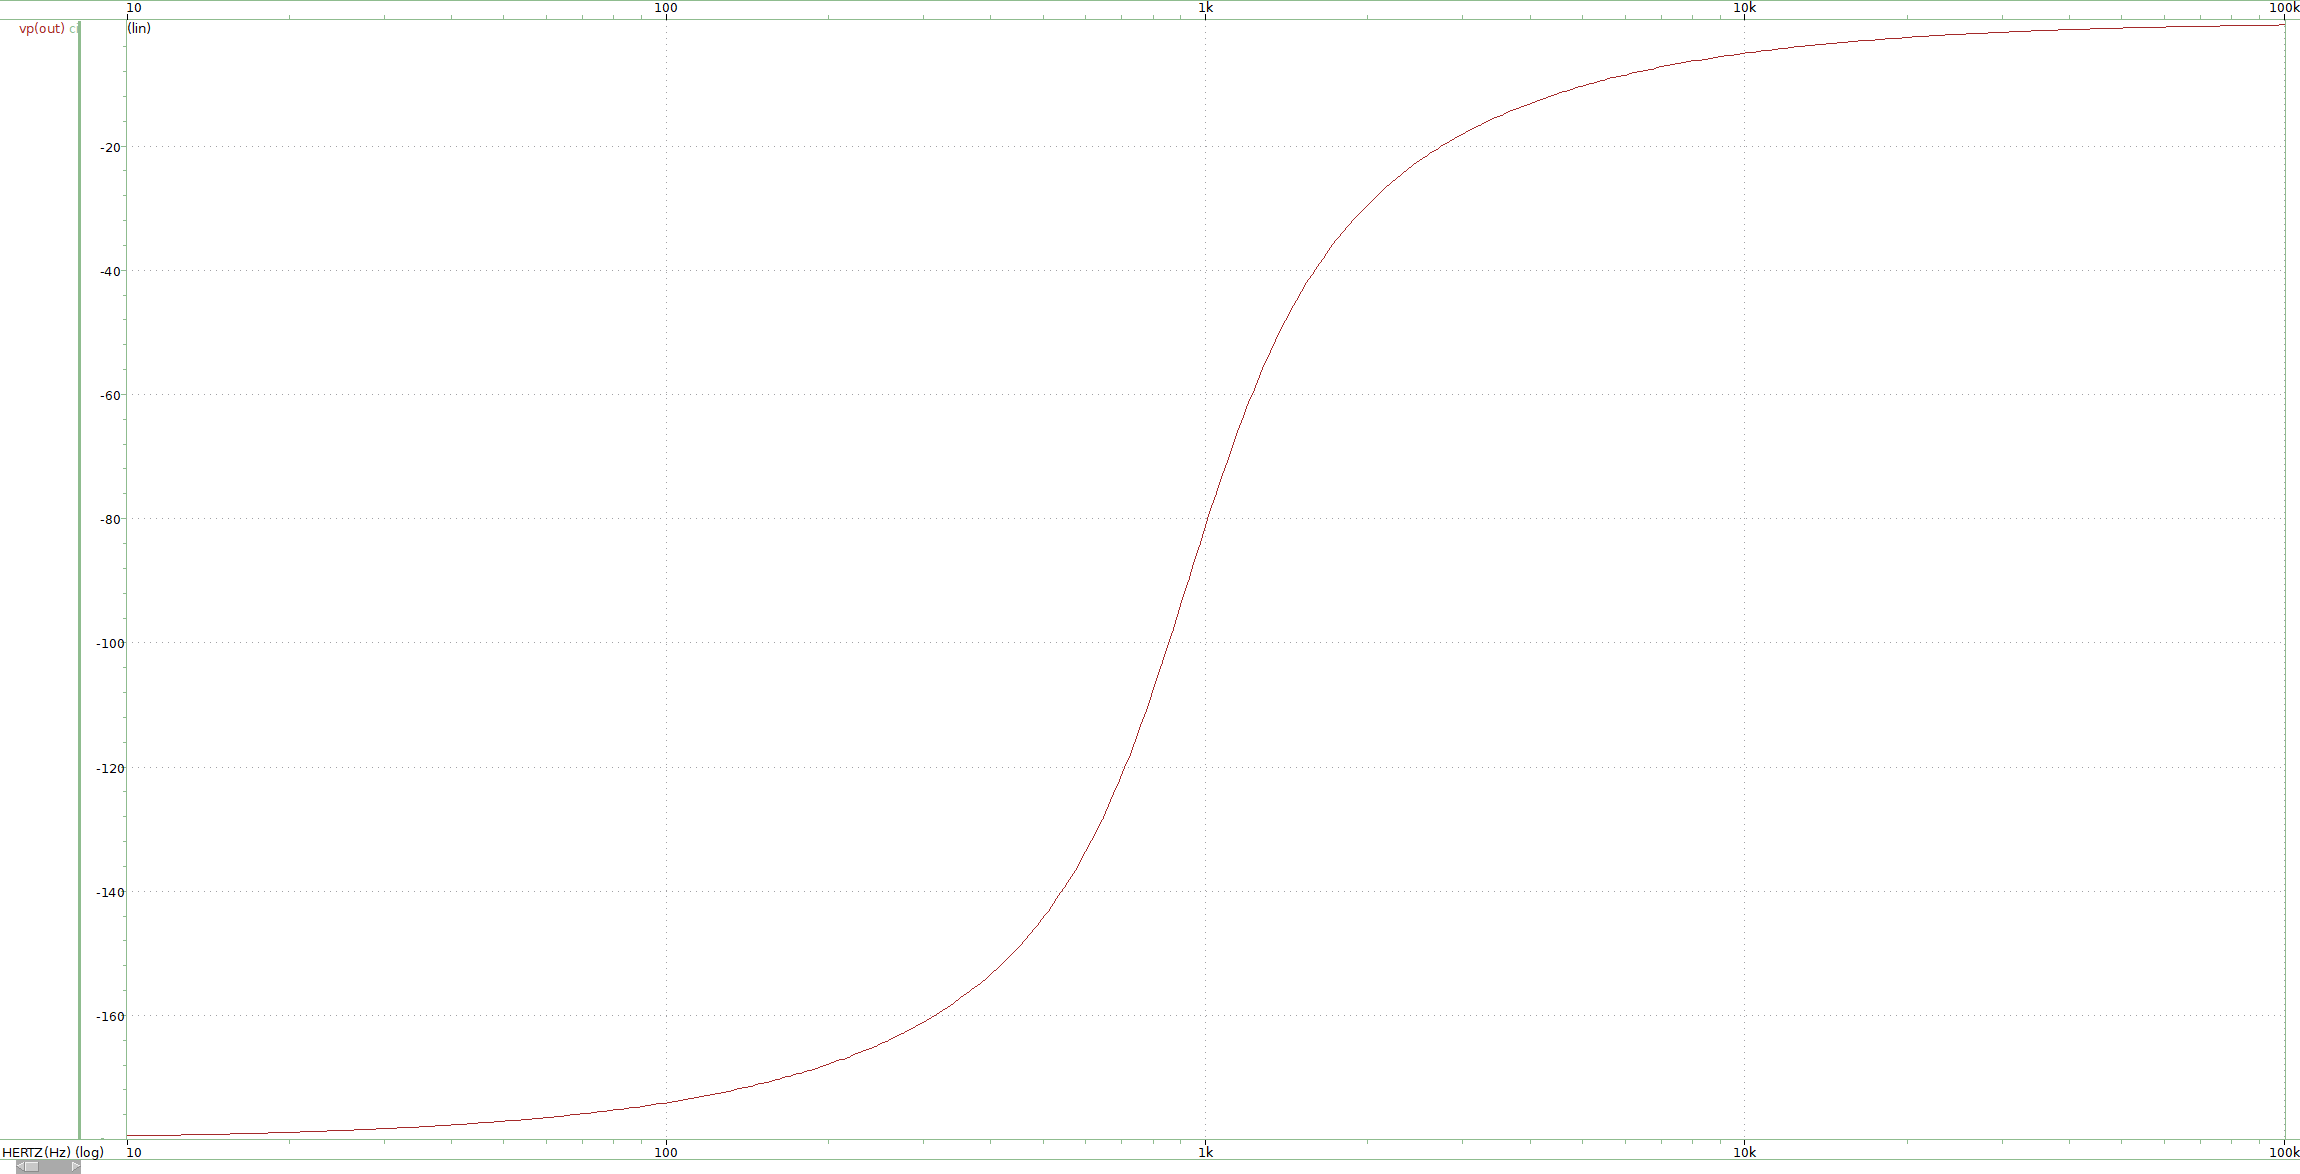
\includegraphics[width=0.8\linewidth]{1_circuito_objetivo_HSPICE/phase_hspice.png}
\caption{Gráfica de Fase de la función de transferencia $H(w)$ obtenida por HSPICE.}
\end{figure}

\begin{figure}[H]
\centering
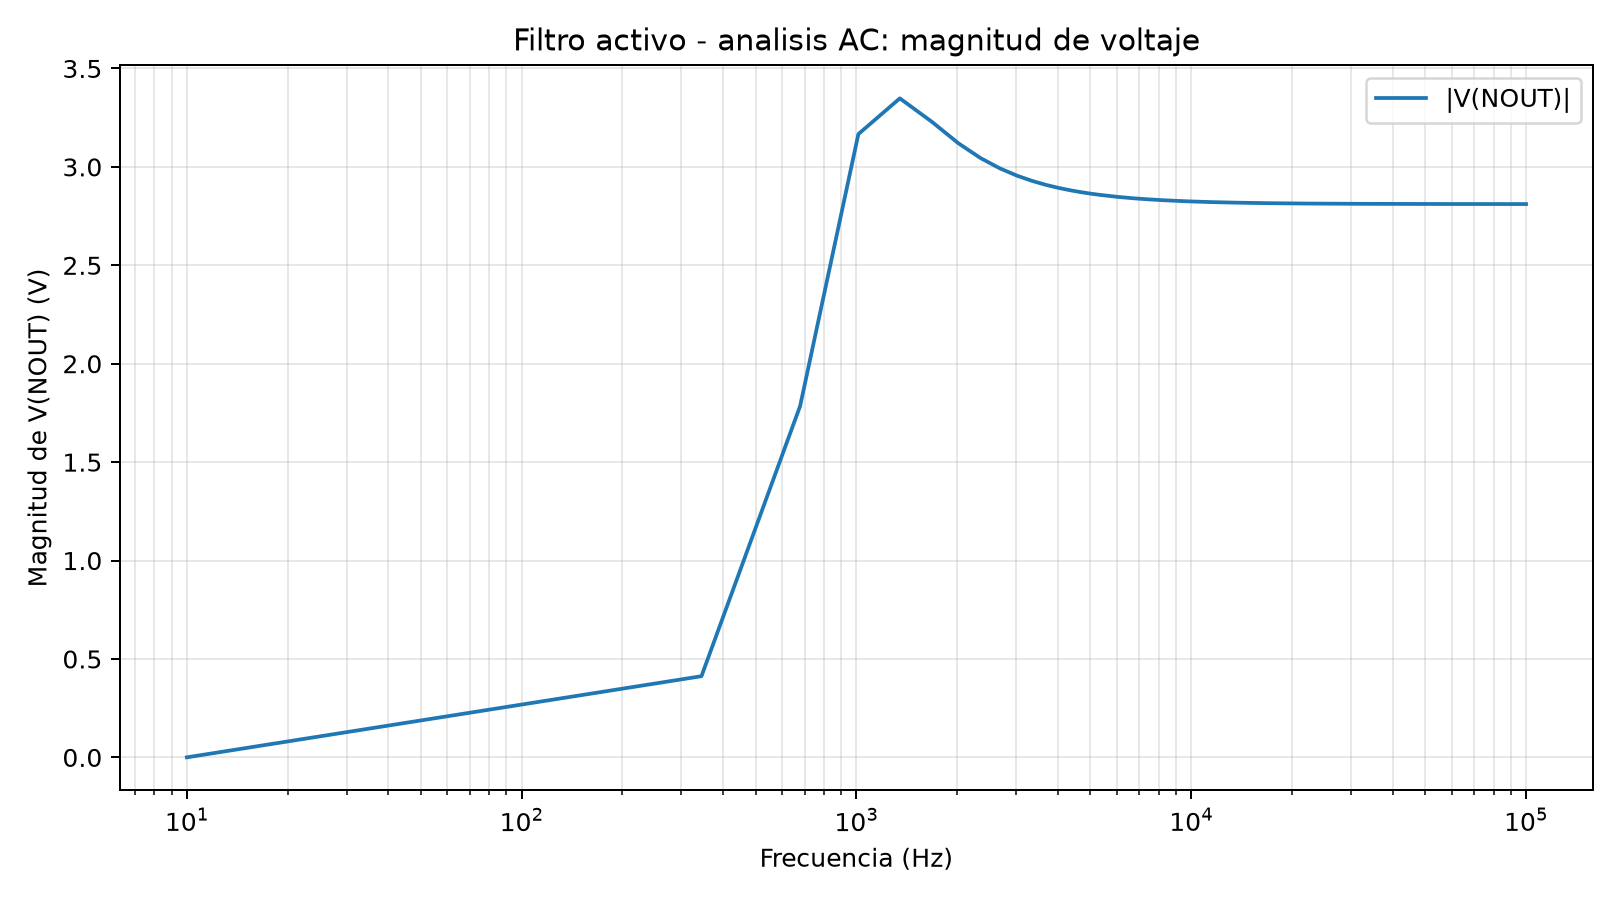
\includegraphics[width=0.75\linewidth]{1_circuito_objetivo_agent/plots/magnitude_voltage.png}
\caption{Gráfica de Magnitud en Voltaje de $V\_OUT$ obtenida por el agente.}
\end{figure}

\begin{figure}[H]
\centering
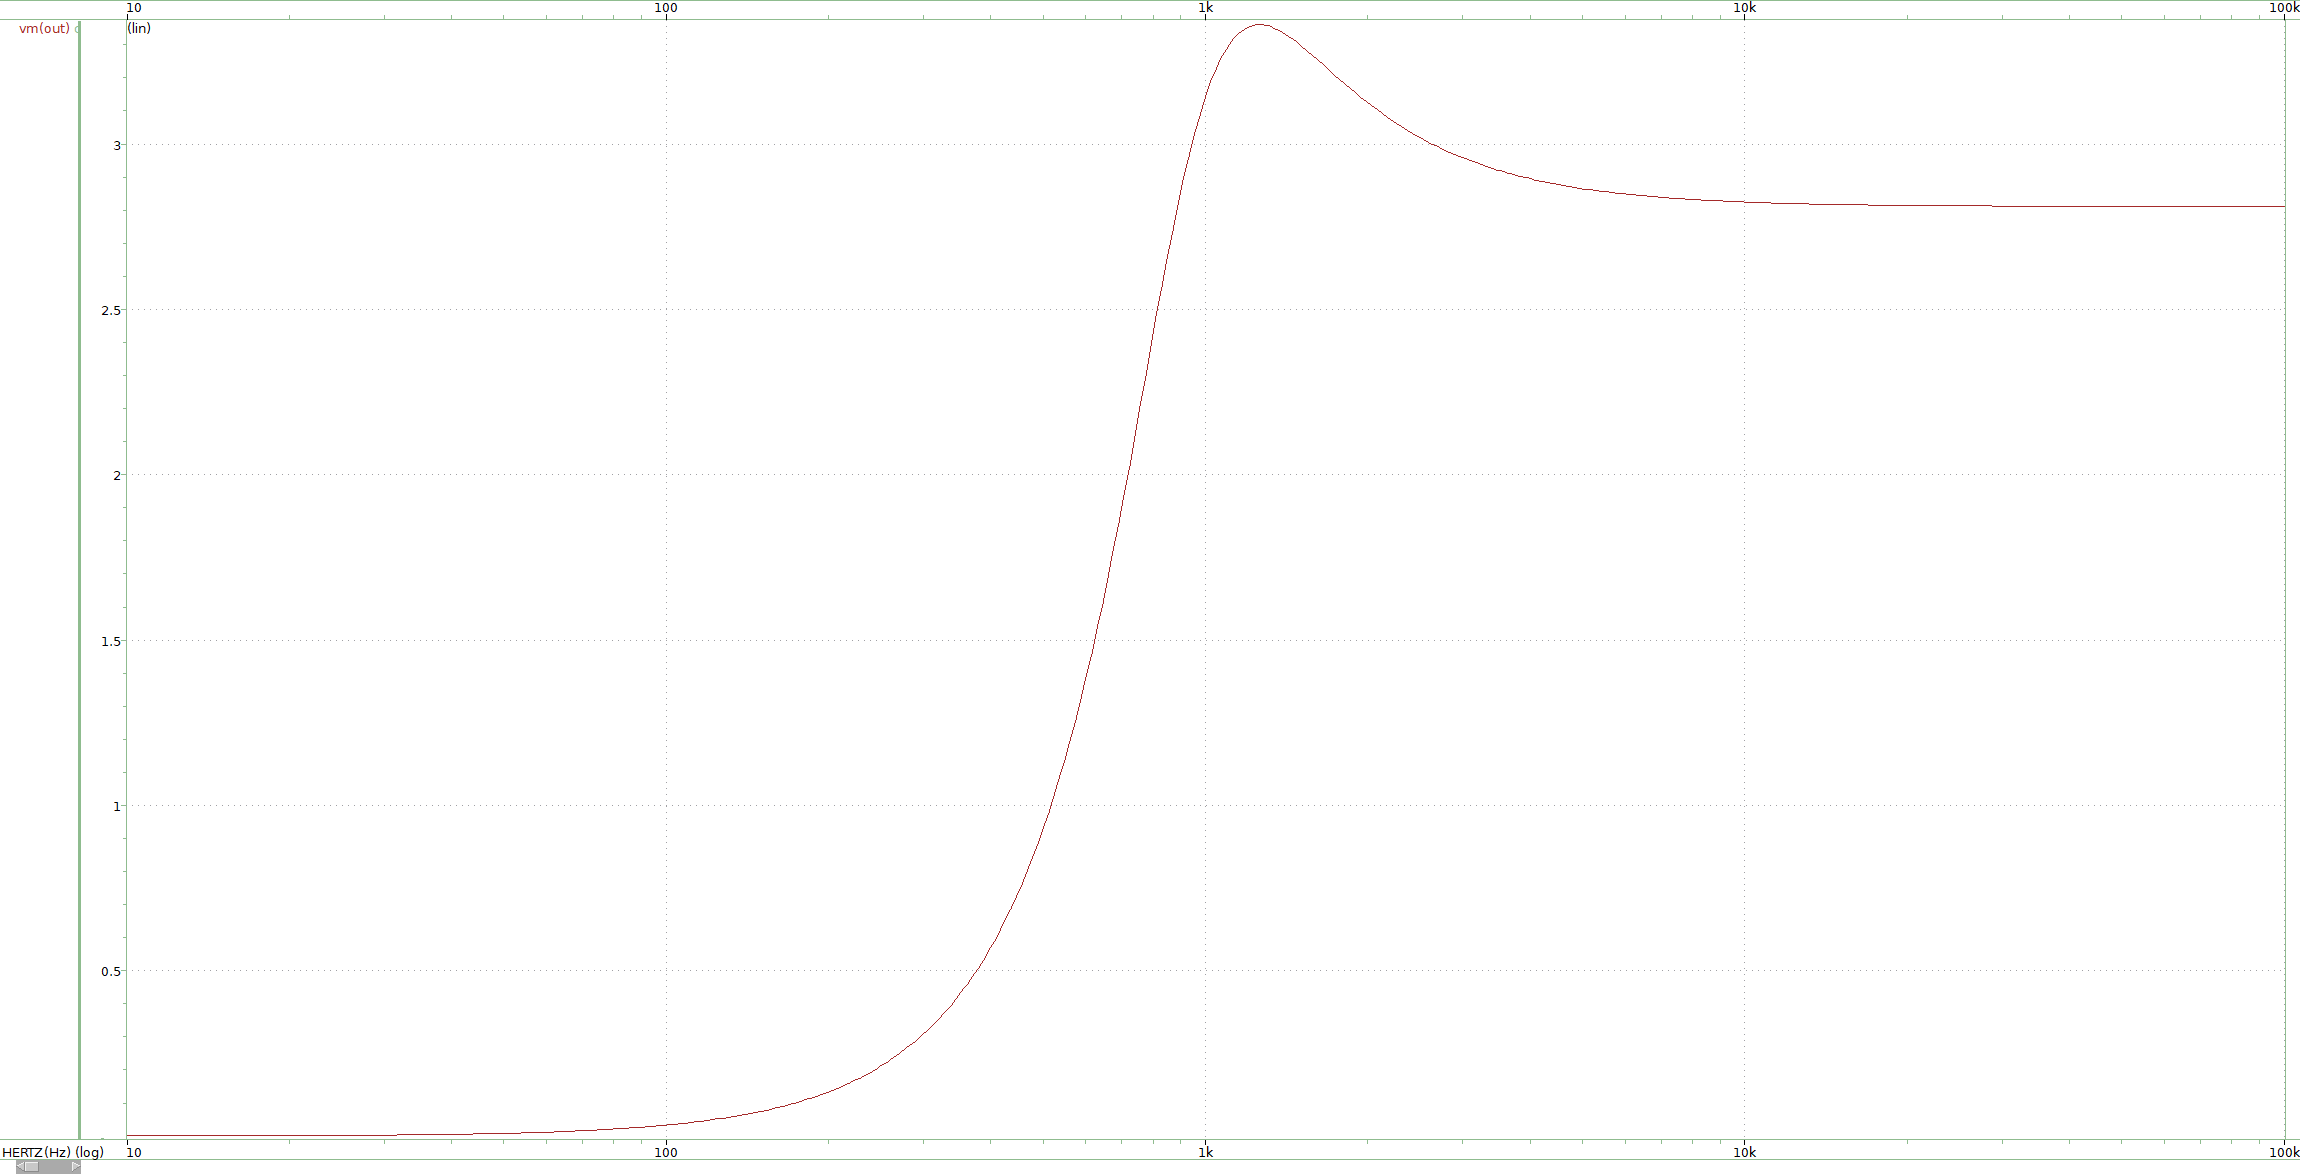
\includegraphics[width=0.75\linewidth]{1_circuito_objetivo_HSPICE/magnitude_voltage_hspice.png}
\caption{Gráfica de Magnitud en Voltaje de $V\_OUT$ obtenida por HSPICE.}
\end{figure}


\subsection{Comparaci\'on con HSPICE}
La comparaci\'on se hizo usando los resultados MNA de \texttt{ac\_results.json} y el listado externo \texttt{circuito\_objectivo\_hspice.lis} (HSPICE V-2023.12-SP2-1). El listado contiene 401 puntos del barrido HSPICE; la ejecuci\'on del agente contiene 300 puntos lineales entre 10 Hz y 100 kHz. La herramienta \texttt{compare\_reference.py} compar\'o \'unicamente las dos frecuencias exactamente coincidentes, 10 Hz y 100 kHz, sin interpolaci\'on. La comparaci\'on usa la transferencia compleja $H(w)$; en los artefactos, el nombre de la referencia \texttt{Vi\_to\_Vo} corresponde al observable \texttt{VOUT\_over\_VIN} del agente.

La comparaci\'on se ejecut\'o con tolerancias absoluta $10^{-6}$ y relativa $2\times10^{-5}$. Los errores de la tabla y los estados proceden de \texttt{compare\_reference.json}; no se calcularon a partir de las gr\'aficas.

\begin{table}[H]
\centering
\begin{tabular}{lccc}
\toprule
Frecuencia & Valor de $H(w)$ del Agente & Valor de $H(w)$ de HSPICE \\
\midrule
10 Hz
& $-3.24160856\times10^{-4} - 3.31084291\times10^{-6}i$
& $-3.24160891\times10^{-4} - 3.31098646\times10^{-6}i$
 \\

100 kHz
& $2.8110469 - 0.0248967i$
& $2.8110897 - 0.0248971i$ \\
\bottomrule
\end{tabular}
\caption{Comparación de la transferencia compleja en los dos puntos con frecuencia exactamente coincidente.}
\end{table}

\begin{table}[H]
\centering
\begin{tabular}{lccccc}
\toprule
Frecuencia & Error absoluto & Error relativo & Estado \\
\midrule
10 Hz
& $1.4771\times10^{-10}$
& $4.5563\times10^{-7}$
& \textbf{PASS} \\

100 kHz
& $4.2845\times10^{-5}$
& $1.5241\times10^{-5}$
& \textbf{PASS} \\
\bottomrule
\end{tabular}


\caption{Comparación de la transferencia compleja en los dos puntos con frecuencia exactamente coincidente.}
\end{table}


El resultado global de la herramienta fue \textbf{Satisfactorio}, dentro de las tolerancias indicadas. La comparaci\'on es limitada: el netlist MNA del agente implementa el op-amp ideal del proyecto, mientras que el deck HSPICE asociado al listado aproxima U1 con una fuente dependiente de ganancia finita $10^9$.